\section{Additional results for \texorpdfstring{\Cref{chap:lifelong}}{}}

\subsection{Bias Analysis}

In this sub-section, we derive a tighter bound than the one provided in \Cref{lem:bias_bound} but with a more intricate expression. 
Notably, this bound also holds for $\omega=1$.

\begin{lemma}
\label{lem:bias_general}
Under \Cref{ass:sce} and \Cref{ass:sch}, the bias of the estimator $\widehat{J}_{T,\alpha,\beta}(\boldsymbol\rho)$, for $0<\omega\leq1$, can be bounded as:
\begin{align*}
    &\left\vert J_{T,\beta}(\boldsymbol\rho) - \mathbb{E}^{\boldsymbol\rho}_{T,\alpha}[\widehat{J}_{T,\alpha,\beta}] \right\vert
    \\
    &\qquad \le\left(L_{\mathcal{M}} + 2\maximumreward L_\nu\right) C_{\gamma}(\beta) \left(\omega 
    \frac{1-\alpha\omega^{\alpha-1} + (\alpha-1) \omega^\alpha}{(1-\omega)(1-\omega^\alpha)} + \frac{1}{1-\gamma}\right),
\end{align*}
where $C_\gamma(\beta)$ is defined as in \Cref{eq:def_function_C}.
In particular, for $\omega=1$, the bound is the limit at $\omega \rightarrow 1$ of the previous expression and reads,
\begin{align*}
    \left|J_{T,\beta}(\boldsymbol\rho) - \mathbb{E}^{\boldsymbol\rho}_{T,\alpha}[\widehat{J}_{T,\alpha,\beta}] \right|\le \left(L_{\mathcal{M}} + 2\maximumreward L_\nu\right) C_{\gamma}(\beta) \left(\frac{\alpha-1}{2} + \frac{1}{1-\gamma}  \right).
\end{align*}
\end{lemma}
\begin{proof}
Recall the definition of $\widehat{J}_{T,\alpha,\beta}(\boldsymbol\rho)$:
\begin{align*}
    \mathbb{E}^{\boldsymbol\rho}_{T,\alpha}\left[\widehat{J}_{T,\alpha,\beta}(\boldsymbol\rho)\right] & = \sum_{t=T-\alpha+1}^T \omega^{T-t}  \int_{\Theta} \nu_{\boldsymbol\rho}(\boldsymbol\theta|t) \frac{\sum_{s=T+1}^{T+\beta} \widehat{\gamma}^s \nu_{\boldsymbol\rho}(\boldsymbol\theta|s)}{\sum_{k=T-\alpha+1}^T \omega^{T-t} \nu_{\boldsymbol\rho}(\boldsymbol\theta|k)} \mathbb{E}_t^{\pi_{\boldsymbol\theta}}[r]  \de \boldsymbol\theta \\
    & = \sum_{s=T+1}^{T+\beta} \widehat{\gamma}^s \int_{\Theta}  \nu_{\boldsymbol\rho}(\boldsymbol\theta|s) \frac{\sum_{t=T-\alpha+1}^T \omega^{T-t} \nu_{\boldsymbol\rho}(\boldsymbol\theta|t) \mathbb{E}_t^{\pi_{\boldsymbol\theta}}[r]  }{\sum_{k=T-\alpha+1}^T \omega^{T-k} \nu_{\boldsymbol\rho}(\boldsymbol\theta|k)} \de \boldsymbol\theta.
\end{align*}
Observe that $J_{T,\beta}(\boldsymbol\rho) = \sum_{s=T+1}^{T+\beta} \widehat{\gamma}^s \int_{\Theta} \nu_{\boldsymbol\rho}(\boldsymbol\theta|s) \mathbb{E}_s^{\pi_{\boldsymbol\theta}}[r] \de \boldsymbol\theta$. 
Therefore,
\begin{align*}
    &\left\vert \mathbb{E}^{\boldsymbol\rho}_{T,\alpha}\left[\widehat{J}_{T,\alpha,\beta}(\boldsymbol\rho)\right] - J_{T,\beta}(\boldsymbol\rho)\right\vert 
    \\
    &\qquad =\left| \sum_{s=T+1}^{T+\beta} \widehat{\gamma}^s \int_{\Theta}  \nu_{\boldsymbol\rho}(\boldsymbol\theta|s) \frac{\sum_{t=T-\alpha+1}^T \omega^{T-t} \nu_{\boldsymbol\rho}(\boldsymbol\theta|t) \mathbb{E}_t^{\pi_{\boldsymbol\theta}}[r]  }{\sum_{k=T-\alpha+1}^T \omega^{T-k} \nu_{\boldsymbol\rho}(\boldsymbol\theta|k)} \de \boldsymbol\theta \right.
    \\
    &\qquad - \left.\sum_{s=T+1}^{T+\beta} \widehat{\gamma}^s \int_{\Theta} \nu_{\boldsymbol\rho}(\boldsymbol\theta|s) \mathbb{E}_s^{\pi_{\boldsymbol\theta}}[r] \de \boldsymbol\theta \right| 
    \\
    &\qquad = \left| \sum_{s=T+1}^{T+\beta} \widehat{\gamma}^s \int_{\Theta}  \nu_{\boldsymbol\rho}(\boldsymbol\theta|s) \frac{\sum_{t=T-\alpha+1}^T \omega^{T-t} \nu_{\boldsymbol\rho}(\boldsymbol\theta|t) \left(\mathbb{E}_t^{\pi_{\boldsymbol\theta}}[r] - \mathbb{E}_s^{\pi_{\boldsymbol\theta}}[r] \right) }{\sum_{k=T-\alpha+1}^T \omega^{T-k} \nu_{\boldsymbol\rho}(\boldsymbol\theta|k)} \de \boldsymbol\theta  \right|.
\end{align*}
Next, by adding and removing the quantity $\textstyle\overline{\nu}(\boldsymbol\theta) \coloneq \frac{1}{C_{\omega}(\alpha)} \sum_{k=T-\alpha+1}^T \omega^{T-k} \nu_{\boldsymbol\rho}(\boldsymbol\theta|k)$, to the last term above, one gets:
\begin{align*}
   &\Bigg| \sum_{s=T+1}^{T+\beta} \widehat{\gamma}^s \int_{\Theta}  \nu_{\boldsymbol\rho}(\boldsymbol\theta|s) \frac{\sum_{t=T-\alpha+1}^T \omega^{T-t} \nu_{\boldsymbol\rho}(\boldsymbol\theta|t) \left(\mathbb{E}_t^{\pi_{\boldsymbol\theta}}[r] - \mathbb{E}_s^{\pi_{\boldsymbol\theta}}[r] \right) }{\sum_{k=T-\alpha+1}^T \omega^{T-k} \nu_{\boldsymbol\rho}(\boldsymbol\theta|k)} \de \boldsymbol\theta  \Bigg|  \\
   &\qquad = \left| \sum_{s=T+1}^{T+\beta} \widehat{\gamma}^s \int_{\Theta}  \left(\nu_{\boldsymbol\rho}(\boldsymbol\theta|s) \pm \overline{\nu}_{\boldsymbol\rho}(\boldsymbol\theta)\right) \frac{\sum_{t=T-\alpha+1}^T \omega^{T-t} \nu_{\boldsymbol\rho}(\boldsymbol\theta|t)  \left(\mathbb{E}_t^{\pi_{\boldsymbol\theta}}[r] - \mathbb{E}_s^{\pi_{\boldsymbol\theta}}[r] \right) }{C_\omega(\alpha) \overline{\nu}(\boldsymbol\rho)} \de \boldsymbol\theta  \right|\\
    &\qquad \le \underbrace{\left| \sum_{s=T+1}^{T+\beta} \widehat{\gamma}^s \int_{\Theta}  \overline{\nu}_{\boldsymbol\rho}(\boldsymbol\theta)  \frac{\sum_{t=T-\alpha+1}^T \omega^{T-t} {\nu}_{\boldsymbol\rho}(\boldsymbol\theta|t) \left(\mathbb{E}_t^{\pi_{\boldsymbol\theta}}[r] - \mathbb{E}_s^{\pi_{\boldsymbol\theta}}[r] \right) }{C_\omega(\alpha) \overline{\nu}(\boldsymbol\rho)} \de \boldsymbol\theta  \right|}_{\text{(a)}} \\
    &\qquad \quad + \underbrace{\left| \sum_{s=T+1}^{T+\beta} \widehat{\gamma}^s \int_{\Theta}  \left(\nu_{\boldsymbol\rho}(\boldsymbol\theta|s) - \overline{\nu}_{\boldsymbol\rho}(\boldsymbol\theta)\right) \frac{\sum_{t=T-\alpha+1}^T \omega^{T-t} \nu_{\boldsymbol\rho}(\boldsymbol\theta|t) \left(\mathbb{E}_t^{\pi_{\boldsymbol\theta}}[r] - \mathbb{E}_s^{\pi_{\boldsymbol\theta}}[r] \right) }{C_\omega(\alpha) \overline{\nu}(\boldsymbol\rho)} \de \boldsymbol\theta  \right|}_{\text{(b)}}.
\end{align*}
We can bound (a) as follows,
\begin{align}
    \text{(a)} & = \frac{1}{C_\omega(\alpha)} \left| \sum_{s=T+1}^{T+\beta} \widehat{\gamma}^s \int_{\Theta}  \sum_{t=T-\alpha+1}^T \omega^{T-t} {\nu}_{\boldsymbol\rho}(\boldsymbol\theta|t) \left(\mathbb{E}_t^{\pi_{\boldsymbol\theta}}[r] - \mathbb{E}_s^{\pi_{\boldsymbol\theta}}[r] \right) \de \boldsymbol\theta  \right| 
    \nonumber\\
    & \le \frac{1}{C_\omega(\alpha)}  \sum_{s=T+1}^{T+\beta} \widehat{\gamma}^s \int_{\Theta}  \sum_{t=T-\alpha+1}^T \omega^{T-t} {\nu}_{\boldsymbol\rho}(\boldsymbol\theta|t) \left|\mathbb{E}_t^{\pi_{\boldsymbol\theta}}[r] - \mathbb{E}_s^{\pi_{\boldsymbol\theta}}[r] \right| \de \boldsymbol\theta  
    \nonumber\\
    &  \le \frac{L_{\mathcal{M}}}{C_\omega(\alpha)}  \sum_{s=T+1}^{T+\beta} \widehat{\gamma}^s  \sum_{t=T-\alpha+1}^T \omega^{T-t} \int_{\Theta} \nu_{\boldsymbol\rho}(\boldsymbol\theta|t) \left|t-s \right|  \de \boldsymbol\theta 
    \label{eq:last_tkt1}\\
    & \le \frac{L_{\mathcal{M}}}{C_\omega(\alpha)}  {\sum_{s=T+1}^{T+\beta} \widehat{\gamma}^s   \sum_{t=T-\alpha+1}^T \omega^{T-t} \left|t-s \right|}, 
    \label{eq:last_tkt2}
\end{align}
where we use the fact that $\textstyle\int_{\Theta} {\nu}_{\boldsymbol\rho}(\boldsymbol\theta|t) \de \boldsymbol\theta = 1$ in \Cref{eq:last_tkt2} and \Cref{ass:sce} in \Cref{eq:last_tkt1}. 
Moving on to (b),
\begin{align}
    (b) & \le 2\maximumreward  \sum_{s=T+1}^{T+\beta} \widehat{\gamma}^s \int_{\Theta}  \left|\nu_{\boldsymbol\rho}(\boldsymbol\theta|s) - \overline{\nu}_{\boldsymbol\rho}(\boldsymbol\theta)\right| \frac{\sum_{t=T-\alpha+1}^T \omega^{T-t} \nu_{\boldsymbol\rho}(\boldsymbol\theta|t) }{C_\omega(\alpha) \overline{\nu}(\boldsymbol\rho)} \de \boldsymbol\theta 
    \nonumber\\
    & = 2\maximumreward  \sum_{s=T+1}^{T+\beta} \widehat{\gamma}^s \int_{\Theta}  \left|\nu_{\boldsymbol\rho}(\boldsymbol\theta|s) - \overline{\nu}_{\boldsymbol\rho}(\boldsymbol\theta)\right|  \de \boldsymbol\theta 
    \nonumber\\
    & \le 2\maximumreward  \sum_{s=T+1}^{T+\beta} \widehat{\gamma}^s  \frac{1}{C_{\omega}(\alpha)} \sum_{t=T-\alpha+1}^{T} \omega^{T-t} \int_{\Theta} \left|\nu_{\boldsymbol\rho}(\boldsymbol\theta|s) - \nu_{\boldsymbol\rho}(\boldsymbol\theta|t) \right|  \de \boldsymbol\theta 
    \nonumber\\
    & \le  \frac{2\maximumreward  L_{\nu}}{C_{\omega}(\alpha)} \sum_{s=T+1}^{T+\beta} \widehat{\gamma}^s   \sum_{t=T-\alpha+1}^{T} \omega^{T-t} \left|t - s \right|,  
    \label{eq:last_tkt3}
\end{align}
where we used \Cref{ass:sch} in \Cref{eq:last_tkt3}.
Regrouping (a) and (b) yields:
\begin{align*}
    \left\vert J_{T,\beta}(\boldsymbol\rho) - \mathbb{E}^{\boldsymbol\rho}_{T,\alpha}[\widehat{J}_{T,\alpha,\beta}] \right\vert \le \frac{L_{\mathcal{M}} + 2\maximumreward L_\nu}{C_\omega(\alpha)} \sum_{s=T+1}^{T+\beta} \sum_{t=T-\alpha+1}^{T} \widehat{\gamma}^s    \omega^{T-t} (s-t).
\end{align*}
The following derivations use a similar structure to \cite[Lemma~3.4]{jagerman2019people}. 
First, setting $m = s-T$ and $n=T-t$, one gets,
\begin{align}
    \frac{1}{C_\omega(\alpha)}\sum_{t=T-\alpha+1}^{T} \omega^{T-t} (s-t)
    &=  \frac{1}{C_\omega(\alpha)}\sum_{n=0}^{\alpha-1} \omega^{n} (m+n) \nonumber\\
    &= m + \frac{1}{C_\omega(\alpha)}
    \sum_{n=1}^{\alpha-1} \omega^{n} n.\label{eq:sum_m_n}
\end{align}
We now study the two following cases. \\
\noindent$\bullet\;$\textbf{Case $\omega<1$.}\indent One has,
\begin{align*}
    \frac{1}{C_\omega(\alpha)}\sum_{t=T-\alpha+1}^{T} \omega^{T-t} (s-t)
    &= m + \frac{1}{C_\omega(\alpha)} \omega \frac{d}{d\omega}
    \sum_{n=1}^{\alpha-1} \omega^{n} 
    \\
    &= m + \frac{1}{C_\omega(\alpha)} \omega 
    \frac{1-\alpha\omega^{\alpha-1} + (\alpha-1) \omega^\alpha}{(1-\omega)^2}
    \\
    &= m + \omega 
    \frac{1-\alpha\omega^{\alpha-1} + (\alpha-1) \omega^\alpha}{(1-\omega)(1-\omega^\alpha)},
\end{align*}
which yields
\begin{align*}
    &\left|J_{T,\beta}(\boldsymbol\rho) - \mathbb{E}^{\boldsymbol\rho}_{T,\alpha}\left[\widehat{J}_{T,\alpha,\beta}\right] \right| 
    \\
    &\qquad \le \frac{L_{\mathcal{M}} + 2\maximumreward L_\nu}{C_\omega(\alpha)} \sum_{s=T+1}^{T+\beta} \sum_{t=T-\alpha+1}^{T} \widehat{\gamma}^s    \omega^{T-t} (s-t) 
    \\
    &\qquad= \left(L_{\mathcal{M}} + 2\maximumreward L_\nu\right) \sum_{s=T+1}^{T+\beta} \widehat{\gamma}^s \left(m + \omega 
    \frac{1-\alpha\omega^{\alpha-1} + (\alpha-1) \omega^\alpha}{(1-\omega)(1-\omega^\alpha)}\right)
    \\
    &\qquad= \left(L_{\mathcal{M}} + 2\maximumreward L_\nu\right) \sum_{s=T+1}^{T+\beta} \widehat{\gamma}^s \left((s-T) + \omega 
    \frac{1-\alpha\omega^{\alpha-1} + (\alpha-1) \omega^\alpha}{(1-\omega)(1-\omega^\alpha)}\right)
    \\
    &\qquad= \left(L_{\mathcal{M}} + 2\maximumreward L_\nu\right)  \left(\frac{1-\gamma^\beta}{1-\gamma}  \omega 
    \frac{1-\alpha\omega^{\alpha-1} + (\alpha-1) \omega^\alpha}{(1-\omega)(1-\omega^\alpha)} + \sum_{k=0}^{\beta-1} \gamma^k (k+1)\right)
    \\
    &\qquad= \left(L_{\mathcal{M}} + 2\maximumreward L_\nu\right)  \left(\frac{1-\gamma^\beta}{1-\gamma}  \omega 
    \frac{1-\alpha\omega^{\alpha-1} + (\alpha-1) \omega^\alpha}{(1-\omega)(1-\omega^\alpha)} + \frac{1-\gamma^\beta}{(1-\gamma)^2}\right)
    \\
    &\qquad= \left(L_{\mathcal{M}} + 2\maximumreward L_\nu\right) \frac{1-\gamma^\beta}{1-\gamma} \left(\omega 
    \frac{1-\alpha\omega^{\alpha-1} + (\alpha-1) \omega^\alpha}{(1-\omega)(1-\omega^\alpha)} + \frac{1}{1-\gamma}\right).
\end{align*}
\noindent$\bullet\;$\textbf{Case $\omega=1$.}\indent Here, \Cref{eq:sum_m_n} becomes:
\begin{align*}
    \frac{1}{C_\omega(\alpha)}\sum_{t=T-\alpha+1}^{T} \omega^{T-t} (s-t)
     = m + \frac{1}{\alpha}
    \sum_{n=1}^{\alpha-1} n = m + \frac{\alpha-1}{2}.
\end{align*}
Thus, the bound becomes:
\begin{align*}
    \left|J_{T,\beta}(\boldsymbol\rho) - \mathbb{E}^{\boldsymbol\rho}_{T,\alpha}\left[\widehat{J}_{T,\alpha,\beta}\right] \right| 
    &\leq \left(L_{\mathcal{M}} + 2\maximumreward L_\nu\right) \sum_{s=T+1}^{T+\beta} \widehat{\gamma}^s \left(m +  \frac{\alpha-1}{2}\right)
    \\
    &= \left(L_{\mathcal{M}} + 2\maximumreward L_\nu\right) \left(C_{\gamma}(\beta)  \frac{\alpha-1}{2} + \sum_{k=0}^{\beta-1}\gamma^k (k+1)  \right) 
    \\
    &= \left(L_{\mathcal{M}} + 2\maximumreward L_\nu\right) C_{\gamma}(\beta) \left(\frac{\alpha-1}{2} + \frac{1}{1-\gamma}  \right). 
\end{align*}
\end{proof}




\subsection{On the Variational Bounds of \Renyi Divergence between Mixture of Distributions}
\label{app:var_bound}
In this appendix, we discuss several upper bounds on the \Renyi divergence $\exponentialrenyidivergence[\alpha](\Psi\left\Vert\Phi\right.)$ between mixtures of distributions $\textstyle\Psi = \sum_{i=1}^L \zeta_i P_i$ and $\textstyle\Phi = \sum_{j=1}^K \mu_j Q_j$ where $\forall i \in [\![1,L]\!],\ j \in [\![1,K]\!],\  0<\zeta_i,\ \mu_j <1$ and $\textstyle\sum_{i=1}^L \zeta_i = \sum_{j=1}^K \mu_j= 1$.
We restrict to the case $\alpha\ge1$. 
First, we report a foundational result from \cite{papini2019optimistic}.

\begin{lemma}[Lemma~4, \cite{papini2019optimistic}]
\label{pp:papini_lemma}
    Consider the sets of variational parameters $\{\psi_{ij}\}_{(i,j)\in[\![1,L]\!]\times [\![1,K]\!]}$ and $\{\phi_{ij}\}_{(i,j)\in[\![1,L]\!]\times [\![1,K]\!]}$, 
    s.t. 
    $\phi_{ij},\psi_{ij}\ge 0$,  $\textstyle\sum_{i=1}^L \psi_{ij} = \mu_j$ and $\textstyle\sum_{j=1}^K \phi_{ij} = \zeta_i$. 
    Then for any $\alpha\ge 1$, and for the mixtures of distributions defined above, one has that,
    \begin{align}
    \label{eq:papini_lemma}
        \exponentialrenyidivergence[\alpha](\Psi\left\Vert\Phi\right.) \leq \sum_{i=1}^L\sum_{j=1}^K \phi_{ij}^{\alpha} \psi_{ij}^{1-\alpha} \exponentialrenyidivergence[\alpha](P_i\left\Vert Q_j\right)^{\alpha-1}.
    \end{align}
\end{lemma}

The search for the tightest upper bound amounts to finding values of $\{\psi_{ij}\}$ and $\{\phi_{ij}\}$ that minimise \Cref{eq:papini_lemma}.
A straightforward but unsuccessful choice would be uniform values. 
In the following, we derive six alternative approaches for the choice of $\{\psi_{ij}\}$ and $\{\phi_{ij}\}$ in order to get a tighter bound. 
Finally, we compare these possible bounds on a toy problem in order to select the best one. 



\subsubsection{Direct Convex Optimisation}
The problem of minimising \Cref{eq:papini_lemma} for $\phi_{ij}\geq 0$ and $\psi_{ij}\geq 0$ under their respective constraints is convex. 
It is therefore possible to take a rather direct approach and use a gradient descent approach to optimise for those variational parameters. 

\textbf{With Reset.}
A first way to do so consists in starting from a uniform distribution over the variational parameters and then following the direction of the gradient for a successive number of steps.
The same process must be applied each time a bound on the \Renyi divergence is required from POLIS. 
We call this approach \emph{direct optimisation with reset}.

\textbf{Without Reset.}
A second idea is to follow the direction of the gradient for a number of successive steps, also, but starting from the previous values of the variational parameters rather than a uniform distribution. 
To be more specific, each time POLIS requires a bound on the \Renyi divergence, the variational parameters of the previous bound are used as starting point for the new optimisation problem. 
We call this approach \emph{direct optimisation without reset}.


\subsubsection{Two Steps Minimisation}
It is not really satisfactory to have to solve an optimisation problem each time an upper bound is required.
In this section, we propose an alternative derivation based on the following theorem.

\begin{thm}[Theorem~5, \cite{papini2019optimistic}]
\label{th:mix_phi}
    Consider a probability distribution $P$ and consider the previous mixture $\Phi$, then for any $\alpha\geq1$, one has:
    \begin{align*}
        \exponentialrenyidivergence[\alpha](P\left\Vert\Phi\right.) \leq     \frac{1}{\sum_{j=1}^K\frac{\mu_j}{\exponentialrenyidivergence[\alpha]( P \Vert Q_j)}}.
    \end{align*}
\end{thm}

Note that the bound involves the harmonic mean of the \Renyi-divergences between $P$ and the mixture's component. 
Similarly, we derive a bound for $\exponentialrenyidivergence[\alpha](\Psi\left\Vert Q\right)$ where $\Psi$ is a mixture.

\begin{prop}
\label{pp:mix_psi}
    Let $Q$ be a probability measure and consider the previous mixture $\Psi$, then for any $\alpha\geq1$, one has:
    \begin{align*}
        \exponentialrenyidivergence[\alpha](\Psi\left\Vert Q\right.) \leq \left(\sum_{i=1}^L \zeta_i \exponentialrenyidivergence[\alpha](P_i\Vert Q)^{\frac{\alpha-1}{\alpha}}\right)^{\frac{\alpha}{\alpha-1}}.
    \end{align*}
\end{prop}
\begin{proof}
Following \cite{papini2019optimistic}, since \Cref{eq:papini_lemma} is convex in $\{\psi_i\}$, one can find the optimal value of $\{\psi_i\}$ using Lagrange multipliers,
\begin{align*}
    \psi_i = \frac{\zeta_i \exponentialrenyidivergence[\alpha](P_i \Vert Q)^{\frac{\alpha-1}{\alpha}}}{\sum_{i=1}^L \zeta_i \exponentialrenyidivergence[\alpha](P_i\Vert Q)^{\frac{\alpha-1}{\alpha}}}.
\end{align*}
Replacing this value in the original problem yields,
\begin{align*}
    \exponentialrenyidivergence[\alpha](\Psi\left\Vert Q\right.)^{\alpha-1} 
    &\leq \sum_{i=1}^L \zeta_i^\alpha \left(\frac{\zeta_i \exponentialrenyidivergence[\alpha](P_i \Vert Q)^{\frac{\alpha-1}{\alpha}}}{\sum_{i=1}^L \zeta_i \exponentialrenyidivergence[\alpha](P_l\Vert Q)^{\frac{\alpha-1}{\alpha}}} \right)^{1-\alpha} \exponentialrenyidivergence[\alpha](P_i \Vert Q)^{\alpha-1}
    \\
    &= \sum_{i=1}^L \zeta_i\frac{ \exponentialrenyidivergence[\alpha](P_i \Vert Q)^{(1-\alpha)\frac{\alpha-1}{\alpha} +\alpha-1}}{\left(\sum_{l=1}^L \zeta_l \exponentialrenyidivergence[\alpha](P_l\Vert Q)^{\frac{\alpha-1}{\alpha}}\right)^{1-\alpha}} 
    \\
    &= \frac{\sum_{i=1}^L \zeta_i \exponentialrenyidivergence[\alpha](P_i \Vert Q)^{\frac{\alpha-1}{\alpha} }}{\left(\sum_{i=1}^L \zeta_i \exponentialrenyidivergence[\alpha](P_i\Vert Q)^{\frac{\alpha-1}{\alpha}}\right)^{1-\alpha}} 
    \\
    &= \left(\sum_{i=1}^L \zeta_i \exponentialrenyidivergence[\alpha](P_i\Vert Q)^{\frac{\alpha-1}{\alpha}}\right)^{\alpha} .
\end{align*}
\end{proof}

In particular, compared to \Cref{th:mix_phi}, this bound now involves the weighted power mean of the exponent $\textstyle\frac{\alpha-1}{\alpha}$ of the \Renyi divergence between $Q$ and the element of the mixture. 
Now, one can combine \Cref{th:mix_phi} and \Cref{pp:mix_psi} to find a bound for $\exponentialrenyidivergence[\alpha](\Psi\left\Vert\Phi\right)$. 
Depending on which result is applied first, different bounds are found.


\textbf{Two Steps $\psi$ First.}
\label{subsubsec:two_steps_psi_first}
Applying \Cref{pp:mix_psi} then \Cref{th:mix_phi} yields the following bound that we refer to as \textit{two steps $\psi$ first}. 

\begin{prop}
\label{pp:var_bound_2_steps_psi_first}
    Under the assumptions of \Cref{pp:papini_lemma}, one has:
    \begin{align*}
        \exponentialrenyidivergence[\alpha](\Psi\left\Vert \Phi\right.) 
        &\leq 
        \left(\sum_{i=1}^L \zeta_i \exponentialrenyidivergence[\alpha](P_i\Vert \Psi)^{\frac{\alpha-1}{\alpha}}\right)^{\frac{\alpha}{\alpha-1}}\\
        &\leq 
        \left(\sum_{i=1}^L \zeta_i \frac{1}{\left(\sum_{j=1}^K\frac{\mu_j}{\exponentialrenyidivergence[\alpha]( P_i \Vert Q_j)}\right)^{\frac{\alpha-1}{\alpha}}}\right)^{\frac{\alpha}{\alpha-1}}.
    \end{align*}
\end{prop}


\renyidivergencebound*
\begin{proof}
    The result follows by applying \Cref{pp:var_bound_2_steps_psi_first} for $\alpha=2$ to the mixtures $\textstyle\sum_{s=T+1}^{T+\beta} \frac{\widehat{\gamma}^s}{C_\gamma(\beta)} \nu_{\boldsymbol\rho}(\cdot|s)$ and $\textstyle\sum_{t=T-\alpha+1}^{T} \frac{\omega^{T-t} }{C_\omega(\alpha)}\nu_{\boldsymbol\rho}(\cdot|t)$.
\end{proof}



\textbf{Two Steps $\phi$ First.}
Alternatively, applying \Cref{pp:mix_psi} first then \Cref{th:mix_phi} yields the following bound which we refer to as \textit{two steps $\phi$ first}.

\begin{prop}
    Under the assumptions of \cref{pp:papini_lemma},
    \begin{align*}
    \exponentialrenyidivergence[\alpha](\Psi\left\Vert \Phi\right.)
    &\leq \frac{1}{\sum_{j=1}^K \frac{\mu_j}{\exponentialrenyidivergence[\alpha](\Psi\Vert Q_j)}}
    \\
    &\leq \frac{1}{\sum_{j=1}^K \mu_j \left(\sum_{i=1}^L \zeta_i \exponentialrenyidivergence[\alpha](P_i\Vert Q_j)^{\frac{\alpha-1}{\alpha}}\right)^{-\frac{\alpha}{\alpha-1}} }.
\end{align*}
\end{prop}

Applying this result to the bound in \Cref{lem:variance_bound} yields the following result.

\begin{prop}[Lower bound with {two steps $\phi$ first}]
    For $\delta>0$, with probability at least $1-\delta$, it holds that 
\begin{align*}
    &\mathbb{E}\left[\overline{J}_{T,\alpha,\beta} \right] 
    \\
    &\qquad\geq 
    \overline{J}_{T,\alpha,\beta} - \sqrt{
            \frac{1-\delta}{\delta} 2\maximumreward}
    \\
    &\qquad\cdot\sqrt{C_\gamma(\alpha)^2 +
            \frac{ C_\omega(\alpha)}{\sum_{ k=T-\alpha+1}^{ T}\omega^{T-k} \left(\sum_{ s=T+1}^{ T+\beta} \widehat{\gamma}^s d_2(\nu_{\boldsymbol\rho}(\cdot\vert s)\Vert \nu_{\boldsymbol\rho}(\cdot\vert k))^{\frac{1}{2}}\right)^{-2} }}.
\end{align*}
\end{prop}


\subsubsection{One Step then Uniform}
In this section, we explore the possibility of solving for one set of variational parameters as a function of the other before replacing its values in \Cref{eq:papini_lemma}. 
In the next proposition, we give the expression of $\{\psi_{ij}\}_{(i,j)\in[\![1,L]\!]\times [\![1,K]\!]}$ as a function of $\{\phi_{ij}\}_{(i,j)\in[\![1,L]\!]\times [\![1,K]\!]}$ and vice-versa.

\begin{prop}
    Under the same assumptions as in \Cref{pp:papini_lemma}, the optimal values of $\psi_{ij}$ are
    \begin{align}
    \label{eq:psi_optim}
        \psi_{ij} = \mu_{j} \frac{\phi_{ij}\exponentialrenyidivergence[\alpha](P_i\Vert Q_j)^{\frac{\alpha-1}{\alpha}}}{\sum_{l=1}^L \phi_{lj}\exponentialrenyidivergence[\alpha](P_l\Vert Q_j)^{\frac{\alpha-1}{\alpha}}};
    \end{align}
    the optimal values of $\phi_{ij}$ are
    \begin{align}
    \label{eq:phi_optim}
        \phi_{ij} = \frac{\zeta_i \psi_{ij}}{ \exponentialrenyidivergence[\alpha](P_i\Vert Q_j)} \left(\sum_{k=1}^K\frac{\psi_{ik}}{\exponentialrenyidivergence[\alpha](P_i\Vert Q_k)}\right)^{-1}.
    \end{align}
\end{prop}
\begin{proof}
    By \Cref{eq:papini_lemma}, one knows that
    \begin{align*}
        \exponentialrenyidivergence[\alpha](\Psi\Vert\Phi)^{\alpha-1}\leq\sum_{i=1}^{L}\sum_{j=1}^K \phi_{ij}^\alpha \psi_{ij}^{1-\alpha} \exponentialrenyidivergence[\alpha](P_i\Vert Q_j)^{\alpha-1}.
    \end{align*}
    The Lagrangian of the problem reads:
    \begin{align*}
        \mathcal{L}(\phi_{ij},\phi_{ij},\lambda_i^{\zeta},\lambda_j^{\mu})=\sum_{i=1}^{L}\sum_{j=1}^K \phi_{ij}^\alpha \psi_{ij}^{1-\alpha} \exponentialrenyidivergence[\alpha](P_i\Vert Q_j)^{\alpha-1} - \sum_{i=1}^L \lambda_i^{\zeta} (\sum_{j=1}^K \phi_{ij} - \zeta_i)
        - \sum_{j=1}^K \lambda_j^{\mu} (\sum_{i=1}^L \psi_{ij} - \mu_j).
    \end{align*}
    Taking the derivative and solving for zero with respect to the variational variables yields,
    \begin{align*}
        \frac{\partial \mathcal{L}}{\partial \phi_{ij}} &= \alpha \phi_{ij}^{\alpha-1} \psi_{ij}^{1-\alpha} \exponentialrenyidivergence[\alpha] (P_i\Vert Q_j)^{\alpha-1}-\lambda_i^{\zeta} =0.
    \end{align*}
    It implies that: 
    \begin{align*}
        \phi_{ij} = \frac{{\lambda_i^{\zeta}}^{\frac{1}{\alpha-1}}\psi_{ij}}{\alpha^{\frac{1}{\alpha-1}} \exponentialrenyidivergence[\alpha](P_i\Vert Q_j)}.
    \end{align*}
    Recall that $\sum_{j}\phi_{ij}=\zeta_i$ so:
    \begin{align*}
        \left(\frac{{\lambda_i^{\zeta}}}{\alpha}\right)^{\frac{1}{\alpha-1}} \sum_{k=1}^K \frac{\psi_{ik}}{\exponentialrenyidivergence[\alpha](P_i\Vert Q_k)} = \zeta_l.
    \end{align*}
    This gives the value of $\lambda_i^{\zeta}$:
    \begin{align*}
        \lambda_i^{\zeta} = \frac{\alpha \zeta_i^{\alpha-1}}{\left(\sum_{k=1}^K\frac{\psi_ik}{\exponentialrenyidivergence[\alpha](P_i\Vert Q_k)}\right)^{\alpha-1}}.
    \end{align*}
    Finally, by replacing,
    \begin{align*}
        \phi_{ij} = \frac{\zeta_i \psi_{ij}}{ \exponentialrenyidivergence[\alpha](P_i\Vert Q_j)} \left(\sum_{k=1}^K\frac{\psi_{ik}}{\exponentialrenyidivergence[\alpha](P_i\Vert Q_k)}\right)^{-1}.
    \end{align*}
    Doing the same for $\psi_{ij}$:
    \begin{align*}
        \frac{\partial \mathcal{L}}{\partial \psi_{ij}} &= (1-\alpha) \psi_{ij}^{\alpha} \psi_{ij}^{-\alpha} \exponentialrenyidivergence[\alpha] (P_i\Vert Q_j)^{\alpha-1}-\lambda_j^{\mu} = 0.
    \end{align*}
    This implies that 
    \begin{align*}
        \psi_{ij} = \left(\frac{1-\alpha}{\lambda_j^{\mu}}\right)^{\frac{1}{\alpha}}\phi_{ij}\exponentialrenyidivergence[\alpha](P_i\Vert Q_j)^{\frac{\alpha-1}{\alpha}}.
    \end{align*}
    Recall that $\sum_{i}\psi_{ij}=\beta_j$ so:
    \begin{align*}
        \left(\frac{1-\alpha}{\lambda_j^{\mu}}\right)^{\frac{1}{\alpha}} \sum_{l=1}^L \phi_{lj}\exponentialrenyidivergence[\alpha](P_l\Vert Q_j)^{\frac{\alpha-1}{\alpha}} = \mu_l.
    \end{align*}
    This gives the value of $\lambda_j^{\beta}$:
    \begin{align*}
        \lambda_j^{\beta} = \frac{1-\alpha}{\mu_j^\alpha}\left(\sum_{l=1}^L \phi_{lj}\exponentialrenyidivergence[\alpha](P_l\Vert Q_j)^{\frac{\alpha-1}{\alpha}}\right)^\alpha .
    \end{align*}
    Finally, by replacing,
    \begin{align*}
        \psi_{ij} = \mu_j \frac{\phi_{ij}\exponentialrenyidivergence[\alpha](P_i\Vert Q_j)^{\frac{\alpha-1}{\alpha}}}{\sum_{l=1}^L \phi_{lj}\exponentialrenyidivergence[\alpha](P_l\Vert Q_j)^{\frac{\alpha-1}{\alpha}}}.
    \end{align*}
\end{proof}


\textbf{Uniform $\psi$.}
In this section, we propose an upper bound for \Cref{eq:papini_lemma} by leveraging the optimal value of $\phi_{ij}$ from \Cref{eq:phi_optim} and injecting it inside \Cref{eq:papini_lemma}. We then set the parameters $\psi_{ij}$ to a uniform value. 
The bound that it yields is given below and we refer to it as \textit{uniform $\psi$}. 

\begin{prop}
Under the assumptions of \Cref{pp:papini_lemma}, one has
    \begin{align*}
        \exponentialrenyidivergence[\alpha](\Psi\vert\Phi)
        &\leq \sum_{i=1}^L \frac{\zeta_i^\alpha}{L^{1-\alpha}}
        \left(
            \sum_{j=1}^K \frac{\mu_j}{\exponentialrenyidivergence[\alpha](P_i \Vert Q_j)}
        \right)^{1-\alpha}.
    \end{align*}
\end{prop}
\begin{proof}
    Injecting \Cref{eq:phi_optim} inside \Cref{eq:papini_lemma} yields,
    \begin{align*}
        \exponentialrenyidivergence[\alpha](\Psi\vert\Phi)
        &\leq \sum_{i=1}^L\sum_{j=1}^K \zeta_i^\alpha \frac{\psi_{ij}}{\exponentialrenyidivergence[\alpha](P_i \Vert Q_j)}
        \left(
            \sum_{k=1}^K \frac{\psi_{ik}}{\exponentialrenyidivergence[\alpha](P_i \Vert Q_k)}
        \right)^{-\alpha}
        \\
        &= \sum_{i=1}^L \zeta_i^\alpha
        \left(
            \sum_{j=1}^K \frac{\psi_{ij}}{\exponentialrenyidivergence[\alpha](P_i \Vert Q_j)}
        \right)^{1-\alpha}.
    \end{align*}
    Then, recalling the constraints $\psi_{ij}\geq 0$ and $\textstyle\sum_{i=1}^L \psi_{ij}=\mu_j$, setting $\psi_{ij}=\frac{\mu_j}{L}$ satisfies these constraints and yields the result.
\end{proof}

As for previous bound, applying this result to \Cref{lem:variance_bound} yields the following result.
    
\begin{prop}[Lower bound with {uniform $\psi$}]
    For $\delta>0$, with probability at least $1-\delta$, it holds that 
    \begin{align*}
        &\mathbb{E}\left[\overline{J}_{T,\alpha,\beta} \right] 
        \\
        &\qquad \geq  \overline{J}_{T,\alpha,\beta} - 
        \sqrt{
            \frac{1-\delta}{\delta} 2  \maximumreward  }
        \\
        &\qquad
        \sqrt{
            C_\gamma(\alpha)^2 +
            \beta C_\omega(\alpha) 
            \sum_{s=T+1}^{T+\beta} \widehat{\gamma}^{2s}
            \left(
                \sum_{k=T-\alpha+1}^T\frac{\omega^{T-k}}{ d_2(\nu_{\boldsymbol\rho}(\cdot\vert s)\Vert \nu_{\boldsymbol\rho}(\cdot\vert k))}
            \right)^{-1}.
        }
    \end{align*}
\end{prop}


\textbf{Uniform $\phi$.}

Similarly as for the previous upper bound, we leverage the optimal value of $\psi_{ij}$ from \Cref{eq:phi_optim} and inject it into \Cref{eq:papini_lemma}. We then set the parameters $\phi_{ij}$ to a uniform value. 
The bound that it yields is given below and we refer to it as \textit{uniform $\phi$}. 

\begin{prop}
Under the assumptions of \Cref{pp:papini_lemma}, one has
    \begin{align*}
        \exponentialrenyidivergence[\alpha](\Psi\vert\Phi)
        &\leq \sum_{j=1}^K \frac{\mu_j^{1-\alpha}}{K^{\alpha}}  \left(\sum_{i=1}^L \zeta_i \exponentialrenyidivergence[\alpha](P_i \Vert Q_j)^{\frac{\alpha-1}{\alpha}}
        \right)^{\alpha}.
    \end{align*}
\end{prop}
\begin{proof}
    Injecting \Cref{eq:phi_optim} inside \Cref{eq:papini_lemma} yields,
    \begin{align*}
        \exponentialrenyidivergence[\alpha](\Psi\vert\Phi)
        &\leq \sum_{i=1}^L\sum_{j=1}^K \mu_j^{1-\alpha} \frac{\phi_{ij}\exponentialrenyidivergence[\alpha](P_i \Vert Q_j)^{\frac{\alpha-1}{\alpha}}}{\left(\sum_{l=1}^L \phi_{lj}\exponentialrenyidivergence[\alpha](P_l \Vert Q_j)^{\frac{\alpha-1}{\alpha}}\right)^{1-\alpha}}
        \\
        &= \sum_{j=1}^K \mu_j^{1-\alpha} \left(\sum_{i=1}^L \phi_{ij}\exponentialrenyidivergence[\alpha](P_i \Vert Q_j)^{\frac{\alpha-1}{\alpha}}
        \right)^{\alpha}.
    \end{align*}
    Then, recalling the constraints $\phi_{ij}\geq 0$ and $\textstyle\sum_{j=1}^K \phi_{ij}=\zeta_i$, setting $\textstyle\phi_{ij}=\frac{\zeta_i}{K}$ satisfies these constraints and yields the result.
\end{proof}
    
As for previous bound, applying this result to \Cref{lem:variance_bound} yields the following result.
    
\begin{prop}[Lower bound with {uniform $\phi$}]
    For $\delta>0$, with probability at least $1-\delta$, it holds that 
    \begin{align*}
        \mathbb{E}\left[\overline{J}_{T,\alpha,\beta} \right] 
        &\geq  \overline{J}_{T,\alpha,\beta} - 
        \sqrt{
            \frac{1-\delta}{\delta} 2 \maximumreward  }
        \\
        &\sqrt{
            C_\gamma(\alpha)^2 +
            \frac{C_\omega(\alpha)}{\alpha^2}
            \sum_{k=T-\alpha+1}^T \frac{1}{\omega^{T-k}} \left(\sum_{s=T+1}^{T+\beta}\widehat{\gamma}^s d_2(\nu_{\boldsymbol\rho}(\cdot\vert s)\Vert \nu_{\boldsymbol\rho}(\cdot\vert k))^{\frac{1}{2}}
            \right)^{2}
        }.
    \end{align*}
\end{prop}




\subsubsection{Comparison of the Bounds}
We have derived 6 bounds for $\overline{J}_{T,\alpha,\beta}(\boldsymbol\rho)$ with different approaches.  
In this section, we explore which result provides the tightest bound and will therefore be used in practice. 
Recall that the objective of the bound is to regularise the policy to avoid extra non-stationarity. 
Therefore, it is expected of the candidate bound that its optimisation would yield a stationary distribution. 

With this in mind, we design the following test.
We consider the following sinusoidal hyper-policy:
\begin{align*}
    \nu(t) = \theta_t = A \sin(\phi t + \psi) + B.
\end{align*}
This simple hyper-policy offers the advantage of clearly measuring the non-stationarity through the scale parameter $A$.
Therefore, as mentioned previously, optimising our candidate lower bound should drive $A$ to 0.
In this test, we optimise only for the variance bound, and the environment is irrelevant. 
For completeness, however, we report that the environment is a contextual bandit, where the context follows a sinusoidal function as well. 


From \Cref{fig:bandit_variational_bound} we see that the most efficient methods when it comes to making the hyper-policy stationary, and thus push $A$ toward 0, are {uniform $\Psi$}, {two steps $\Psi$ first}, \textit{two steps $\Phi$ first} and the \textit{direct optimization with reset}.

From the results reported in \Cref{fig:bandit_variational_bound} one can see that the upper-bound (right plot) is coarser for approaches based on convex optimisation. 
A second observation is that the upper-bound is tighter for {uniform $\Psi$} and {two steps $\Psi$ first} and also offers a faster convergence of the parameter $A$ toward 0. 
These bounds have similarities but ones needs to make a choice to provide a surrogate objective.
We chose {two steps $\Psi$ first} as we believe that it may be more versatile.
Indeed, using a uniform distribution to set some of the variational parameters as is done for uniform $\Psi$ seems to be not robust to any scenario.

\begin{figure}[t]
    \centering
    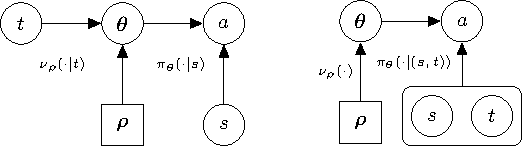
\includegraphics[labellifelong=variationalbound, width=\linewidth]{img/thesis_plots_chapter_lifelong.pdf}
    \caption{\textbf{Left:} Evolution of the scale parameter for several approaches on the upper-bounds of the variance. Note that the value of A for the \textit{two steps $\Psi$ first} and \textit{uniform $\Psi$} are confounded.\\
    \textbf{Right:} Evolution of the variational upper-bound on the variance for several approaches. Here again, the log upper-bound for the \textit{two steps $\Psi$ first} and \textit{uniform $\Psi$} are confounded.}
    ``CO'' stands for convex optimisation.
    \label{fig:bandit_variational_bound}
\end{figure}


\subsection{Experimental Details}

\subsubsection{Datasets}
\label{subsubsec:datasets_lifelong}
Here, more details are given on the processes involved in the Trading and the Dam tasks. 
For the Dam, the three mean inflows are represented in \Cref{fig:dam_inflows}.
We also provide the weights to compute the total cost in this environment.
For flooding and not meeting demand, the costs for the first inflow profile are respectively 0.3 and 0.7; for the second inflow profile, 0.8 and 0.2; for the third inflow profile, 0.35 and 0.65.
For the Trading, the historical value of the EUR-USD pair is given in \Cref{fig:eurusd_dataset}.


\begin{figure*}[t]
  \centering
  \begin{subfigure}{.29\textwidth}
  \centering
  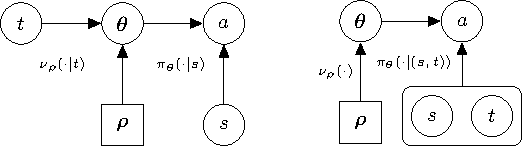
\includegraphics[labellifelong=inflowdam,width=1.3\linewidth]{img/thesis_plots_chapter_lifelong.pdf}
    \end{subfigure}%
  \caption{The three water inflow profiles considered for the Dam experiment.}
  \label{fig:dam_inflows}
\end{figure*}


\begin{figure*}[t]
\centering
\begin{subfigure}{.29\textwidth}
  \centering
  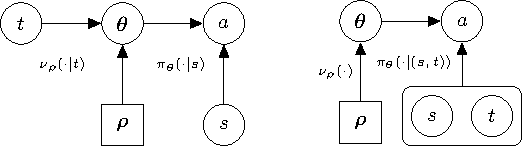
\includegraphics[labellifelong=forexseed0,width=1.3\linewidth]{img/thesis_plots_chapter_lifelong.pdf}
          \caption*{Dataset 2009-2012.}
\end{subfigure}%
\hfill
\begin{subfigure}{.29\textwidth}
  \centering
  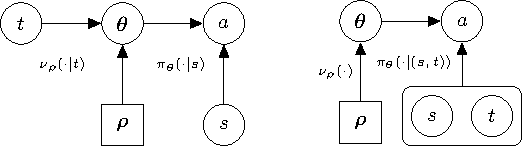
\includegraphics[labellifelong=forexseed1,width=1.3\linewidth]{img/thesis_plots_chapter_lifelong.pdf}
          \caption*{Dataset 2013-2016.}
\end{subfigure}%
\hfill
\begin{subfigure}{.29\textwidth}
  \centering
  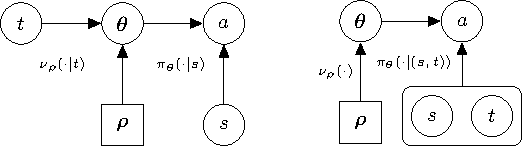
\includegraphics[labellifelong=forexseed2,width=1.3\linewidth]{img/thesis_plots_chapter_lifelong.pdf}
    \caption*{Dataset 2017-2020.}
\end{subfigure}%
\captionof{figure}{Historical exchange rates of the EUR-USD pair for the period 2009-2020 and divided into three datasets.}\label{fig:eurusd_dataset}
\end{figure*}

